\section{Ensemble et correction de prior par Sinkhorn}\label{sec:sinkhorn}

\subsection{Ensemble}
Pour $M$ modèles de probabilités $P^{(m)}\in\Delta_K^{N}$, on prend la moyenne arithmétique
\begin{equation}
\bar P=\frac1M\sum_{m=1}^MP^{(m)} .
\end{equation}
Au run 1, les membres sont \code{signature} et \code{signature\_robust}, chacun avec deux graines. La moyenne simple ne demande aucune sélection de poids sur la validation : celle-ci reste donc un score propre du blend. Deux diagnostics accompagnent l'ensemble :
\begin{equation}
\text{accord}(m,m')=\frac1N\sum_i\ind{\arg\max P^{(m)}_i=\arg\max P^{(m')}_i},\qquad
\text{oracle}=\frac1N\sum_i\ind{\exists m:\arg\max P^{(m)}_i=y_i}.
\end{equation}
Un accord faible et un oracle élevé indiquent des erreurs complémentaires, donc un ensemble utile.

\subsection{Le symptôme}
Sur le test, les 81\,600 prédictions $\arg\max\bar P_i$ se répartissent entre 1\,320 (titre 2) et 7\,112 (titre 7). Un test équilibré en contiendrait $81\,600/24=3\,400$ par titre (figure~\ref{fig:counts}). Les titres sur-prédits (7, 13, 19, 15) sont ceux dont la profondeur est la plus faible au train, et le test est moins profond. Le décalage de covariables se traduit donc en un \emph{biais de prior des prédictions}.

\begin{figure}[H]\centering
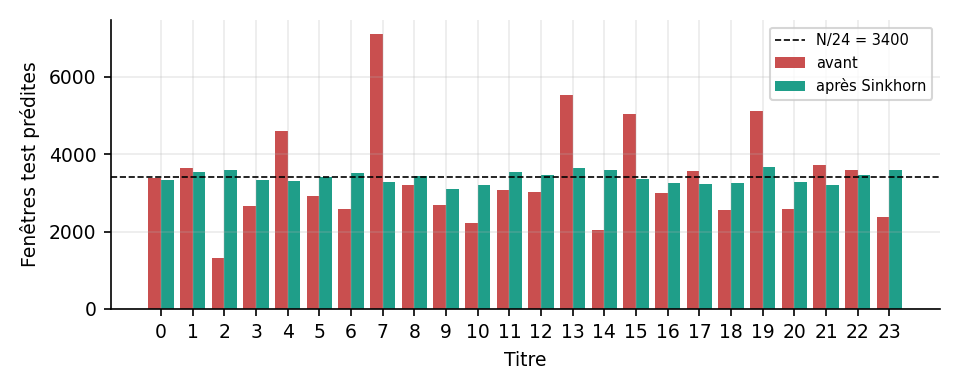
\includegraphics[width=.85\linewidth]{figures/sinkhorn_counts.png}
\caption{Fenêtres test prédites par titre, avant et après équilibrage (blend des 4 finalistes, refit).}
\label{fig:counts}
\end{figure}

\subsection{Rappel : correction de prior sous \emph{label shift}}
Supposons que seule la loi des classes change entre la source $s$ et la cible $\mathrm{t}$, et que $p_s(x\mid y)=p_{\mathrm{t}}(x\mid y)$. Par la formule de Bayes,
\begin{equation}
p_{\mathrm{t}}(y\mid x)=\frac{p(x\mid y)\pi_{\mathrm{t}}(y)}{\sum_{y'}p(x\mid y')\pi_{\mathrm{t}}(y')}
=\frac{p_s(y\mid x)\,\dfrac{\pi_{\mathrm{t}}(y)}{\pi_s(y)}}{\sum_{y'}p_s(y'\mid x)\,\dfrac{\pi_{\mathrm{t}}(y')}{\pi_s(y')}} .
\label{eq:labelshift}
\end{equation}
La correction optimale est donc un \emph{coefficient par classe} $w_y=\pi_{\mathrm{t}}(y)/\pi_s(y)$, suivi d'une renormalisation \cite{saerens,lipton}. Ici, $\pi_s$ est uniforme (6\,700 fenêtres par titre) et $\pi_{\mathrm{t}}$ l'est très probablement aussi. Le problème n'est donc pas un vrai label shift. Mais le covariate shift fait se comporter le modèle \emph{comme si} son prior implicite avait changé. On cherche les coefficients qui ramènent la masse prédite au prior visé.

\subsection{Formulation : projection entropique sur les marges}
Soit $P\in\R_{>0}^{N\times K}$ (probabilités strictement positives, écrêtées à $10^{-12}$), et $r=\1_N$, $c=\frac NK\1_K$ les marges visées. On cherche
\begin{equation}
Q^\star=\arg\min_{Q\ge0}\ \mathrm{KL}(Q\,\|\,P)=\sum_{i,k}Q_{ik}\log\frac{Q_{ik}}{P_{ik}}-Q_{ik}+P_{ik}
\quad\text{s.c.}\quad Q\1_K=r,\ \ Q^\top\1_N=c .
\label{eq:kl}
\end{equation}
\begin{proposition}[Forme de la solution]\label{prop:sinkform}
Il existe $u\in\R^N_{>0}$ et $w\in\R^K_{>0}$ tels que $Q^\star_{ik}=u_i\,P_{ik}\,w_k$.
\end{proposition}
\begin{proof}
Lagrangien : $\mathcal{L}=\mathrm{KL}(Q\|P)+\sum_i a_i(\sum_kQ_{ik}-1)+\sum_kb_k(\sum_iQ_{ik}-N/K)$. La condition de stationnarité donne $\partial\mathcal{L}/\partial Q_{ik}=\log(Q_{ik}/P_{ik})+a_i+b_k=0$, soit $Q_{ik}=P_{ik}e^{-a_i}e^{-b_k}$. On pose $u_i=e^{-a_i}$ et $w_k=e^{-b_k}$. Le problème est strictement convexe sur un polytope non vide (il contient $Q=\frac1K\1\1^\top$), donc la solution est unique.
\end{proof}

\begin{corollaire}[Règle de décision]
$\arg\max_kQ^\star_{ik}=\arg\max_kP_{ik}w_k$. Le facteur de ligne $u_i$ ne change pas la décision : l'équilibrage revient exactement à multiplier chaque titre par un coefficient $w_k$, comme dans~\eqref{eq:labelshift}.
\end{corollaire}

\begin{proposition}[Qui bascule]
La fenêtre $i$, prédite $c$ avant correction, est prédite $c'\neq c$ après si et seulement si
\begin{equation}
\frac{P_{ic'}}{P_{ic}}>\frac{w_c}{w_{c'}}\quad\text{et}\quad c'=\arg\max_kP_{ik}w_k .
\end{equation}
\end{proposition}
\noindent Une fenêtre confiante ($P_{ic}\gg P_{ic'}$) ne bascule que si le rapport des coefficients est extrême. Les fenêtres hésitantes basculent vers leur second choix. C'est ce qu'on observe (figure~\ref{fig:changed}).

\subsection{Algorithme de Sinkhorn--Knopp}
\begin{algo}[H]
\caption{\code{sinkhorn\_balance}}
\begin{algobox}
\item $Q\leftarrow\max(P,10^{-12})$.
\item Répéter 50 fois :
\begin{itemize}
\item[] colonnes : $Q_{ik}\leftarrow Q_{ik}\cdot\dfrac{N/K}{\sum_jQ_{jk}}$ ;
\item[] lignes : $Q_{ik}\leftarrow Q_{ik}\Big/\sum_{k'}Q_{ik'}$.
\end{itemize}
\item Retourner $Q$.
\end{algobox}
\end{algo}
Chaque étape est une projection de Bregman (en divergence KL) sur l'un des deux ensembles de contraintes affines. Pour une matrice strictement positive, les itérations convergent vers l'unique $Q^\star$ de la Proposition~\ref{prop:sinkform} \cite{sinkhorn,cuturi}. Les produits cumulés des facteurs de colonnes donnent $w$, ceux des facteurs de lignes donnent $u$.

\subsection{Exemple complet}
Quatre fenêtres, deux titres, vérité $(A,A,B,B)$.
\begin{center}\small
\begin{tabular}{cccccc}
\toprule
Fenêtre & Vrai & $P$ (A ; B) & avant & $Q^\star$ (A ; B) & après\\
\midrule
1 & A & 0,90 ; 0,10 & A & 0,838 ; 0,162 & A\\
2 & A & 0,70 ; 0,30 & A & 0,573 ; 0,427 & A\\
3 & B & 0,60 ; 0,40 & \old{A} & 0,463 ; 0,537 & \new{B}\\
4 & B & 0,20 ; 0,80 & B & 0,126 ; 0,874 & B\\
\midrule
\multicolumn{2}{c}{masse} & 2,40 ; 1,60 & 3/4 & 2,00 ; 2,00 & 4/4\\
\bottomrule
\end{tabular}
\end{center}
Coefficients obtenus : $w_B/w_A=1{,}739$. La fenêtre 3 bascule car $0{,}40/0{,}60=0{,}667>1/1{,}739=0{,}575$. La fenêtre 2 ne bascule pas : $0{,}30/0{,}70=0{,}43<0{,}575$.

\subsection{Effet observé sur le test}
\begin{figure}[H]\centering
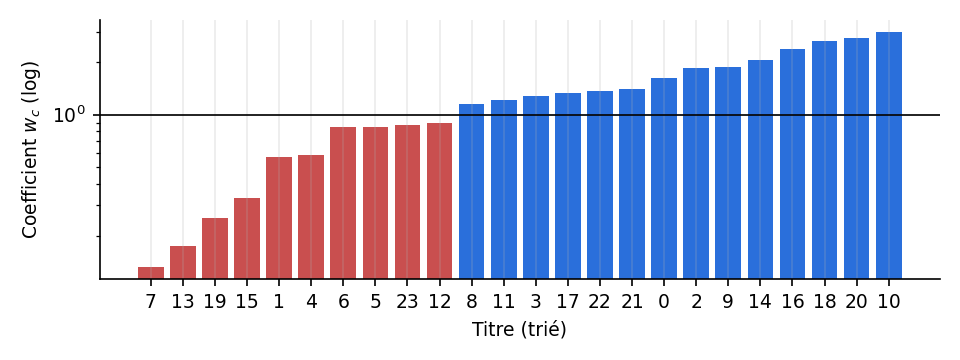
\includegraphics[width=.85\linewidth]{figures/sinkhorn_weights.png}
\caption{Coefficients $w_k$ (normalisés en moyenne géométrique). Titre 7 : $\times0{,}13$ ; titre 10 : $\times2{,}99$.}
\end{figure}
\begin{figure}[H]\centering
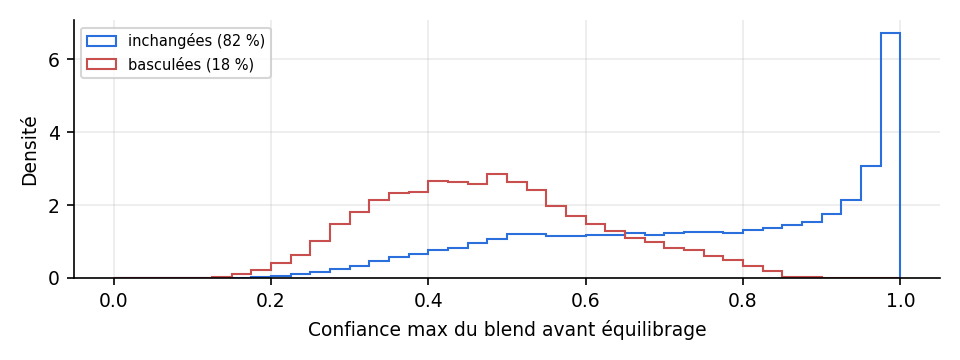
\includegraphics[width=.85\linewidth]{figures/sinkhorn_changed.png}
\caption{18\,\% des prédictions basculent. Leur confiance moyenne avant correction est de 0,48, contre 0,75 pour les fenêtres inchangées.}
\label{fig:changed}
\end{figure}

\begin{table}[H]\centering\small
\begin{tabular}{lccc}
\toprule
Blend des 4 finalistes & valid & stress & LB public\\
\midrule
brut & 0,8525 & 0,7411 & 0,5700\\
équilibré & 0,8599 & 0,8055 & \textbf{0,5958}\\
\midrule
gain & +0,7 pt & +6,4 pts & +2,6 pts\\
\bottomrule
\end{tabular}
\caption{L'équilibrage a été validé sur le stress \emph{avant} d'être soumis. Le stress, lui-même décalé en profondeur, a correctement prédit le signe du gain au LB, mais pas son ampleur.}
\end{table}

\subsection{Conditions de validité}
\begin{enumerate}
\item \textbf{Test équilibré.} Si $\pi_{\mathrm{t}}$ n'était pas uniforme, imposer $c=\frac NK\1$ dégraderait le score. Le gain observé au LB plaide pour l'uniformité, sans la démontrer.
\item \textbf{Bon classement relatif.} La correction ne change que l'importance relative des titres. Elle répare les fenêtres dont le bon titre est un second choix proche, pas les erreurs confiantes.
\item \textbf{Transductivité.} $w$ dépend de \emph{tout} le test. La prédiction d'une fenêtre dépend donc des autres fenêtres du test, et la conformité au règlement est à vérifier. Une variante non transductive consisterait à estimer $w$ sur un ensemble de référence (le stress, par exemple). Elle serait moins adaptée au vrai décalage.
\item \textbf{Différence avec Saerens et al.} \cite{saerens} \emph{estiment} $\pi_{\mathrm{t}}$ par EM :
\begin{equation}
\pi^{(k+1)}_c=\frac1N\sum_i\hat p^{(k)}_{ic},\qquad \hat p^{(k)}_{ic}\propto P_{ic}\,\pi^{(k)}_c/\pi_s(c).
\end{equation}
Nous \emph{imposons} au contraire que la masse prédite soit uniforme. C'est une hypothèse plus forte, adaptée à un test construit avec 20 fenêtres par titre et par jour.
\end{enumerate}
